\chapter{Conceptos teóricos}

En este apartado se explicaran el grueso de los conceptos necesarios para la correcta comprensión del trabajo y el material. Teniendo tanto en cuenta el funcionamiento de los mecanismos internos como los conceptos abstractos.

\section{Visión e imágenes}
Se empezará definiendo lo que se entiende por imágenes y como se componen estas. Una imagen es una representación visual de un objeto, escena o perspectiva, ya sea de forma física (como una fotografía) o digital (como una imagen digital). Para comprender cómo se compone una imagen, es crucial explicar el funcionamiento de la visión humana.

La visión \cite{formaciongraficaModeloRGB} es un proceso complejo que se produce cuándo determinados fotorreceptores en el interior de nuestros ojos, llamados conos y bastones, reciben la luz reflejada de los objetos, esta luz reflejada para que sea visible por nuestros ojos tiene que venir reflejada entre los valores de frecuencia de 460 nanómetros (nm) y 780 nm, correspondiente al espectro visible para el ojo humano. 

Dentro de este rango, existen tres tipos de conos, cada uno sensible a una parte del espectro: los conos largos, que detectan las frecuencias del rojo, con una longitud de onda entre 618 y 780 nm; los conos medios, que detectan las frecuencias del verde, con una longitud de onda entre 529 y 497 nm; y los conos cortos, que detectan las frecuencias del azul, con una longitud de onda entre 460 y 482 nm. Estas tres señales se combinan en nuestro cerebro, permitiéndonos percibir una amplia gama de colores.

Así los colores que nosotros somos capaces de percibir son una conjunción de los distintos grados de activación de esos tres tipos de sensores, es decir, los distintos colores que interpretamos son una combinación de Rojo, Verde y Azul, por lo tanto el modelo de color que contempla esta composición se llama RGB, por los nombres en inglés de \textit{Red, Green and Blue}.

Esto es relevante para este trabajo ya que nos permite comprender como las imágenes digitales se representan, ya que estas se componen de tres capas o canales, cada uno correspondiente a una de las bandas del espectro RGB. La combinación de estos tres canales permite reproducir la gama de colores que percibimos en la realidad.

Aunque estas capas solo son una selección de las frecuencias reflejadas por como funciona el ojo humano, pero realmente existen otros tipos de radiación electromagnética que se encuentran fuera de este espectro visible.Algunas de estas radiaciones pueden ser captadas por sensores especializados y utilizadas en diversos campos, como la teledetección y la investigación científica.

Concretamente en este trabajo se utiliza una banda más, de una longitud de onda mayor que el rojo, es decir una frecuencia infrarroja. El satélite Sentinel 2 es capaz de recoger hasta 13 bandas\cite{gisgeographySentinelBands}, con distintas resoluciones y longitudes de onda, de las cuales se utilizaran 4 y una composición entre varias de ellas:
 \begin{itemize}
	\item\textbf{Banda 2}: Esta banda es la correspondiente al color azul, con una frecuencia de onda de 490 nm.
	
	\item\textbf{Banda 3}: Esta banda es la correspondiente al color verde, con una frecuencia de onda de 560 nm.
	
	\item\textbf{Banda 4}: Esta banda es la correspondiente al color rojo, con una frecuencia de onda de 665 nm.
	
	\item\textbf{Banda 8}: Esta banda es la correspondiente al una frecuencia infrarroja de 842 nm. Esta banda es relevante ya que a esa frecuencia de onda la luz no se refleja correctamente en la clorofila, por tanto te permite saber el estado de la vegetación de la zona.
	
	\item\textbf{Banda NDVI}: Esta es una combinación de bandas, NDVI son las siglas para \textit{Normalized Difference Vegetation Index}, esta es muy útil para diferenciar zonas en función de la vegetación que poseen, la formula es: 
	
	\begin{math}
	NDVI=\frac{B8-B4}{B8+B4}
	\end{math}
	
\end{itemize}

 Estas bandas, al ser combinadas y procesadas, permiten obtener información valiosa sobre las características y el estado de la superficie terrestre, lo cual es fundamental para los objetivos de este trabajo.
 
\section{Inteligencia artificial}
Dentro de esta sección se explicará algunos modelos de inteligencia artificial y su funcionamiento además de conceptos teóricos básicos para entender esta materia.
La inteligencia artificial \cite{rouhiainen2018inteligencia} consiste en programas capaces de usar algoritmos para aprender de unos datos y ser capaz de tomar decisiones en base a ellos.

La inteligencia artificial se usa en la actualidad para multitud de tareas:

\begin{itemize}
	\item Reconocimiento de imágenes estáticas, clasificación y .
	
	\item Mejoras del desempeño de la estrategia algorítmica comercial.
	
	\item Procesamiento eficiente y escalable de datos de pacientes.
	
	\item Detección y clasificación de objetos.
	
	\item Distribución de contenido en las redes sociales
	
	\item Protección contra amenazas de seguridad cibernética
	
\end{itemize}

El aprendizaje automático o \textit{Machine Learning}\cite{ibmQuMachine} es uno de los principales enfoques de la inteligencia artificial, este utiliza algoritmos para aprender de conjuntos de datos. Este se divide en tres categorías de manera principal:

\begin{itemize}
	\item\textbf{Aprendizaje supervisado}: En este tipo de aprendizaje los algoritmos usan datos previamente etiquetados, es decir que ya tienen una categoría asignada. Esto hace que el modelo a entrenar extraiga las distintas características que convierten el dato de entrada en la categoría de salida. Este tipo de algoritmos se utilizan para la predicción y clasificación de datos. Este es el que se ha utilizado para este trabajo. El deep learning se encuadra dentro de este apartado. Algunos de los métodos más utilizados de este tipo de aprendizaje son las redes neuronales, los clasificadores bayesianos, la regresiones lineales, los bosques aleatorios y las máquinas de vectores de soporte.
	
	\item\textbf{Aprendizaje no supervisado}: En este tipo de aprendizaje se utilizan algoritmos para analizar y agrupar datos no etiquetados. En estos los algoritmos descubren patrones ocultos a simple vista y agrupaciones sin necesidad de intervención humana. Se utilizan para clasificación y agrupación por lo tanto. Entre sus usos se encuentra el análisis exploratorio de datos, la segmentación de datos, el reconocimiento de patrones e incluso la reducción de la dimensionalidad. Algunos métodos utilizados son el análisis de componentes principales, la descomposición en valores singulares, El algoritmo de K-medias y métodos de agrupación probabilística.
	
	\item\textbf{Aprendizaje semisupervisado}:  Este es una variante intermedia a los anteriores, dónde en el entrenamiento se utilizan datos etiquetados sobre un conjunto de datos mayor dónde el resto están sin etiquetar, este te ayuda a etiquetarlos.

\end{itemize}

También cabe destacar el Aprendizaje por refuerzo, el cual funciona como un mecanismo de condicionamiento operante, dónde al algoritmo se le entrena sobre la marcha validando si ha realizado la predicción correcta o no y ajustando este su algoritmo interno para aprender en función de esto.

Es relevante comprender para el contexto de este trabajo que en la clasificación de imágenes binaria, como es la que se da, las etiquetas consisten en una capa de la imagen, llamada \textit{ground truth}, con los valores de 0 y 1 para cada pixel en función de la salida esperada.

\subsection{Métricas de aprendizaje supervisado}
La evaluación de estos modelos de aprendizaje supervisado se puede hacer con diversos métodos, aunque las medidas más básicas son las que se detallaran en este apartado.

La base de todas las métricas\cite{themachinelearnersMtricasClasificacin} que se van a detallar es la \textbf{matriz de confusión}. Esta se compone por cuatro valores en una matriz 2 x 2.
Estos valores son:
\begin{itemize}
	\item True Positives: Este está en la primera posición de la matriz, se corresponde con el número de predicciones que han sido predichas como positivas de manera correcta. En adelante se llamará TP. 
	
	\item True Negatives: Este está en la última posición de la matriz, se corresponde con el número de predicciones que han sido predichas como negativos de manera correcta. En adelante se llamará TN. 
	
	\item False Positives: Este está en la segunda posición de la matriz, se corresponde con el número de predicciones que han sido predichas como positivas de manera incorrecta
	
	\item False Negatives: Este está en la primera posición de la matriz, se corresponde con el número de predicciones que han sido predichas como negativas de manera 
	
\end{itemize}

Ahora se explicarán el resto de medidas, que se calculan sobre los datos de la matriz de confusión.

\subsubsection{Accuracy}
Esta es la principal medida. La precisión representa el porcentaje total de valores correctamente clasificados sobre el total de valores. Esta medida es útil cuando los datos están balanceados. La formula por tanto es:
\begin{equation}
	Accuracy=\frac{TP+TN}{TP+TN+FP+FN}
\end{equation}
 
\subsection{Precisión}
Esta medida de mayor valor a los valores TP, ya que lo que nos plantea es que porcentaje de valores han sido correctamente calificados como positivos sobre todos los valores calificados como positivos. La fórmula por tanto es:

\begin{equation}
	Precisión=\frac{TP}{TP+FP}
\end{equation}

\subsubsection{Recall}
La métrica de recall, es el ratio de verdaderos positivos y sirve para saber cuántos de los valores positivos han sido correctamente clasificados. La formula por tanto es:
\begin{equation}
	Recall=\frac{TP}{TP+FN}
\end{equation}

\subsubsection{F1 Score}
Esta métrica es útil en conjuntos de datos desbalanceados. Esta combina el recall y la precisión. La formula es:
\begin{equation}
	F1 Score=2*\frac{recall*precision}{recall+precision}
\end{equation}

Estás son las métricas que se han utilizado para medir este proyecto, aunque hay otras médidas muy usadas que también definiré.

\subsubsection{Curva ROC}
La curva ROC (Receiver Operating Characteristic) es un gráfico muy utilizado para problemas de clasificación. Esta representa el porcentaje de verdaderos positivos contra el ratio de falsos positivos. Lo que diferencia a esta métrica de las demás es que el umbral por el que se clasifica un elemento como 0 o 1 se va modificando para generar todosl los valores de la gráfica.

\subsubsection{AUC}
Esta métrica es derivada de la anterior, la métrica AUC (Area Under Curve) o área bajo la curva. El valor de esta métrica está entre 0 y 1 siendo 0 una clasificación aleatoria y 1 una clasificación perfecta. Esta se calcula mediante integrales.

\section{Algunos modelos de Inteligencia artificial}

Ahora se explicarán en profundidad algunos de los algoritmos previamente mentados, concretamente los relacionados con este trabajo. 

\subsection{KNN}
KNN\cite{ibmQuKNN} son las siglas para \textit{K Nearest Neighbours}, es decir k vecinos más cercanos, este clasificador de aprendizaje supervisado utiliza la proximidad para hacer clasificaciones o predicciones, aunque generalmente se suele utilizar para clasificación. 

KNN forma parte de la familia de algoritmos de aprendizaje perezoso, ya que en la fase de entrenamiento no realiza cálculos, sino que almacena las instancias, realizándose estos cálculos en la fase de predicción.

También por su funcionamiento se le considera basado en instancias.

Es un algoritmo popular debido a su simplicidad y precisión pero no escalan bien sus capacidades con el crecimientos del conjunto de datos.

Este asigna una etiqueta en función de un calculo de distancia con las instancias del modelo, por lo que uno de los conceptos más relevantes dentro de este modelo son las métricas de distancia, que definirán cuánto se de lejos están unas instancias a otras.

Las ventajas y desventajas de este algoritmo son:

\textbf{Ventajas}:

\begin{itemize}
	\item{Facilidad de implementación}: Como se ha visto el algoritmo es relativamente sencillo.
	
	\item{Gran adaptabilidad}: Ya que al introducir siempre nuevas instancias da una mayor versatilidad.
	
	\item{Pocos hiperparámetros}: Ya que los unicos parámetros que requiere son el valor de K y la medida de distancia.
\end{itemize}

\textbf{Desventajas}:

\begin{itemize}
	\item{Mal escalado}: Como ya se ha comentado, cuándo el número de instancias crece ralentiza la predicción del modelo y hace que requiera más recursos, al tener que cargar en memoria las instancias.
	
	\item{Mal funcionamiento para alta dimensionalidad}: Aumentando el número de errores acorde a la dimensionalidad.
	
	\item{Propensión al sobreajuste}: Por su funcionamiento tiende a sobreajustarse en función del valor k, en especial si es muy baj, pero en caso de tener un k muy alto tiende a ajustarse mal alos datos 
	
\end{itemize}

Su funcionamiento consiste en calcular la distancia de la nueva instancia con el resto de las del modelo y entre las k más cercanas ver que clase es la mayoritaria, esta será la clase predicha.

Algunas de las métricas mas usadas para el cálculo de distancias son:

\begin{itemize}
	\item\textbf{Distancia euclidiana}: Está es de las más utilizadas. Se calcula la distancia de la línea recta entre dos puntos mediante la formula:
	\begin{equation}
		d(a,b)=\sqrt{\sum_{i=1}^{n}(b_{i}-a_{i})^{2}}
	\end{equation}
	n = número de dimensiones del punto.
	
	\item\textbf{Distancia Manhattan}: Esta es una medida más sencilla que mide la distancia entre dos puntos tomando  como trayectoria los vértices del eje. Su formula es:
	\begin{equation}
		d(a,b)=\sum_{i=1}^{n}|a_{i}-b_{i}|
	\end{equation}
	n = número de dimensiones del punto.
	
	\item\textbf{Distancia minkowski}: Esta es la utilizada en el experimento. Es la generalización de las dos anteriores, siendo la p en Manhattan  1 y en la euclídea 2. La formula por tanto es:
	\begin{equation}
		d(a,b)=(\sum_{i=1}^{n}|a_{i}-b_{i}|^p)^{\frac{1}{p}}
	\end{equation}
	n = número de dimensiones del punto.
	
	\item\textbf{Distancia de hamming}:  Esta técnica es utilizada de forma normal para vectores booleanos o cadenas, buscando identificar igualdades i diferencias. Es el sumatorio de los items diferentes.
	
\end{itemize}

Se utiliza entre otros usos para:

\begin{itemize}
	\item{Preprocesamiento de datos}
	
	\item{Finanzas}
	
	\item{Cuidado de la salud}
	
	\item{Reconocimiento de patrones} 
		
\end{itemize}

\subsection{Random Forest}
Random Forest\cite{ibmWhatRandom} o árboles aleatorios es un algoritmo supervisado basado en la combinación de diversos árboles de decisión binarios para alcanzar un único resultado.

Es un algoritmo popular debido a su flexibilidad y facilidad de uso.

Para comprender el Random Forest es necesario comprender antes los árboles de decisión simples, ya que este es una composición de ellos.

Los árboles de decisión binarios se basan en respuestas binarias a preguntas, dónde separan en ramas u hojas los caminos en función de si esa repuesta lleva a otra pregunta (rama) o a una clasificación final (hoja). De esta manera, a base de condiciones se van clasificando las distintas instancias que le llegan al árbol. Las ramas se pueden configurar para definir cuales son las condiciones que se consultan en cada rama, aunque son propensos a problemas como sesgos y sobreajustes. Estos suelen cubrir todo el espacio de posibilidades.

Es un método de aprendizaje por conjuntos, por lo tanto se compone de varios clasificadores que se agregan para identificar el resultado más popular. Estos se entrenan de manera independiente y después se promedian los resultados.

Ahora, el algoritmo del Random Forest consiste en muchos arboles binarios con características aleatorias, es decir con condicionantes aleatorios. Estos por lo tanto no tienen porque cubrir todo el espacio de probabilidades.

El algoritmo del Random Forest tiene tres hiperparámetros principales, el tamaño del nodo, la cantidad de arboles y la cantidad de características muestreadas.

Dependiendo del tipo de problema, la determinación de la predicción variará. Para una tarea de regresión, se promediarán los árboles de decisión individuales, y para una tarea de clasificación, un voto mayoritario, es decir, la variable categórica más frecuente, arrojará la clase predicha.

Las ventajas y desventajas de este modelo son:

\textbf{Ventajas}:

\begin{itemize}
	\item{Bajo riesgo de sobreajuste}: si bien anivel interno se pueden sobreajustar los arboles de decisión al haber gran cantidad de ellos el modelo no se ajusta demasiado al modelo, ya que el promedio de árboles no correlacionados reduce la varianza general y el error de predicción.
	
	\item{Gran flexibilidad}: es un metodo popular porque funciona de manera eficiente tanto para regresiones como clasificaciones.
	
	\item{Facilita la obtención de la importancia de las características}: la evaluación de la importancia o contribución de las variables al modelo. Hay algunas formas de evaluar la importancia de las características. La importancia de Gini y la disminución media de impurezas (MDI) se utilizan generalmente para medir cuánto disminuye la precisión del modelo cuando se excluye una variable determinada.
	
\end{itemize}

\textbf{Desventajas}:

\begin{itemize}
	\item{Puede tardar}: Para grandes conjuntos de datos puede ser relativamente lento.
	
	\item{Requiere de recursos}: Para conjuntos de datos grandes puede requerir de recursos para almacenarlos.
	
	\item{Relativamente opaco}: La predicción de un árbol pouede ser mucho más simple de interpretar que la de un bosque
	
\end{itemize}

Se utiliza entre otros usos para:

\begin{itemize}
	\item{Comercio electrónico}
	
	\item{Finanzas}
	
	\item{Cuidado de la salud}
	
\end{itemize}

\subsection{Máquinas de vectores de soporte (SVM)}

Si bien esta técnica se ha demostrado no ser adecuada para su utilización en este trabajo, al requerir de un tiempo de entrenamiento excesivo, se explicará al haber sido una de las pruebas realizadas.

Una máquina se vectores de soporte\cite{ibmWhatSupport}, en adelante SVM siendo estas las siglas de \textit{Support Vector Machine},  es un algoritmo de aprendizaje automático supervisado que clasifica los datos encontrados en una línea o hiperplano óptimo que maximice la distancia entre cada clase en un espacio N-dimensional. Esto significa que clasifican encontrando lo que diferencia a unas clases de otras dentro de un espacio vectorial en el que se representan las características de unas instancias etiquetadas.

Estos se suelen utilizar en problemas de clasificación. La cantidad de características del modelo marca la dimensionalidad del mismo y por tanto de los propios planos que genera como separación.

Este es capaz de clasificar tanto de manera lineal como no lineal, pero en caso de separar linealmente se suelen utilizar funciones kernel para transformar los datos a un espacio de mayor dimensionalidad para permitir la separación lineal. Se pueden elegir distintos tipos de kernel.

Hay 3 tipos de SVM:

\subsubsection{SVM Lineales}
Estos utilizan datos linealmente separables, por lo que no se necesitan transformaciones para separarlos en diferentes clases. El limite de decisión  ha de tener una separación máxima con las clases. 


Hay dos enfoques para calcular este margen, con un margen duro y con un margen blando, diferenciándose por que en la primera opción todos los puntos están separados por el vector, mientra que en la segunda hay un margen de holgura.

\subsubsection{SVM no lineales}
Normalmente los escenarios del mundo real no son linealmente separables, para poder separarlos se aplica preprocesamiento de datos mediante funciones de kernel para transformarlos en un espacio de características de mayor dimensión. Estas funciones se conocen como "kernel trick". Las hay de diversos tipos como pueden ser kernels lineales, kernels polinomiales, kernels\textit{Radial Basis function}(RBF) o kernels sigmoides. Esto aumenta el riesgo de sobreajuste.

\subsubsection{Regresión de vectores de soporte (SVR)}
La regresión de vectores de soporte es una extensión de las SVM dedicada a los problemas de regresión. Si las SVM encuentran el vector o plano que separa los datos las SVR tratan de encontrar el vector o plano que siguen los datos.


\subsection{Redes neuronales}
En este apartado se explicarán los modelos que quedan por mentar que siendo estas, las redes neuronales, las redes neuronales convolucionales y finalmente la red U-Net, que es un tipo de red neuronal convolucional. 

Una red neuronal\cite{ibmQuNeuronal} es un modelo de machine learning las cuales tienen un fundamento similar a las neuronas biológicas.

Las redes neuronales son un conjunto de neuronas, compuestas por una o varias neuronas en la capa de entrada, una o varias capas ocultas intermedias y finalmente una capa de salida. 

El funcionamiento de una neurona es el siguiente:
\begin{enumerate}
	\item Se asignan una ponderaciones a los distintos valores de entrada de la neurona.
	
	\item Estas ponderaciones se multiplican por el valor de su entrada y se suman
	
	\item La suma se pasa a través de una función de activación dónde se determina la salida de la neurona
	
	\item Si esta salida es superior al valor umbral de la neurona esta se activa y pasa señal a la siguiente capa.
	
\end{enumerate}
Al entrenar el algoritmo se quiere evaluar su precisión utilizando una función de coste o pérdida, la cual tiene la neurona la misión de minimizar.

El modelo va ajustando su ponderaciones y valores umbral utilizando la función de coste y el aprendizaje reforzado para alcanzar un punto de convergencia.

Las redes neuronales también pueden tener retropropagación, es decir la actualización de los pesos y el umbral viene marcada por las capas posteriores.

Las redes neuronales se entrenan y mejoran su precisión con el tiempo.

Si bien Deep learning y redes neuronales son términos que se usan indistintamente de forma general, pero en verdad solo se consideran deep learning si hay más de 3 capas.

\subsubsection{Tipos}
Existen distintos tipos de redes neuronales, que se usan para fines diferentes. Aunque aquí se explicaran las más comunes:

\begin{itemize}
	\item{Perceptrón simple}:esta es una red neuronal con una capa de 1 neurona de entrada, un salida de 1 neurona y sin capas ocultas o intermedias.
	
	\item{Redes neuronales de avance}: o perceptrones multicapa, se componen de una capa de entrada, una o varias capas ocultas y una capa de salida.
	
	\item{Redes neuronales recurrentes}: Tienen bucles de retroalimentación. Estas se emplean datos de series temporales para hacer predicciones futuras.
	
	\item{redes neuronales convolucionales}	: Estás se definirá en más profundidad en el próximo apartado. don redes neuronales hacia adelante (feedforward) y se utilizan para reconocimiento de imágenes Estas utilizan la multiplicación de matrices y los principios del álgebra lineal.
\end{itemize}

\subsection{Redes neuronales convolucionales}\label{sect:redesConvolucionales}
Como ya se ha mentado, son un subtipo de redes neuronales\cite{ibmQuRedes}, usualmente utilizadas para tareas de clasificación y reconocimiento de imágenes. Son un enfoque escalable para tareas de clasificación de imágenes y reconocimiento de objetos. Estas pueden requerir altos recursos computacionales.

Estas tienen tres tipos de capas:
\begin{itemize}
	\item{Capa convolucional}
	
	\item{Capa de agrupación}
	
	\item{Capa totalmente conectada}	
\end{itemize}

La red siempre empieza por una capa de convolución y acaba por una capa totalmente conectada, aunque después de la primera capa de convolución pueden ir otras capas convolucionales o capas de agrupación. Cada capa del modelo aumenta la complejidad de la red, identificando partes cada vez más grandes. Las primeras capas se centran en características simples como bordes y colores. 

\subsubsection{Capa convolucional}
Esta es el bloque de creación principal de la red y se realizan en ella la mayoría de los cálculos. Requiere de datos de entrada, un filtro y un mapa de características. También hay un detector de característica, el filtro, el cual se encarga de comprobar si esa característica está presente en los datos de entrada.

El detector de características es una matriz, normalmente bidimensional de 3x3, esto determina el tamaño del campo receptivo. Después se aplica este filtro a un área de la imagen calculando el producto escalar entre el filtro y  los datos de entrada. Esto va a la matriz de salida y se repite el proceso sobre toda la imagen. La capa resultante se denomina mapa de características, mapa de activación o característica convolucionada. Se puede ver en la figura~\ref{fig:filtro}.

\begin{figure}[H]
	\centering
	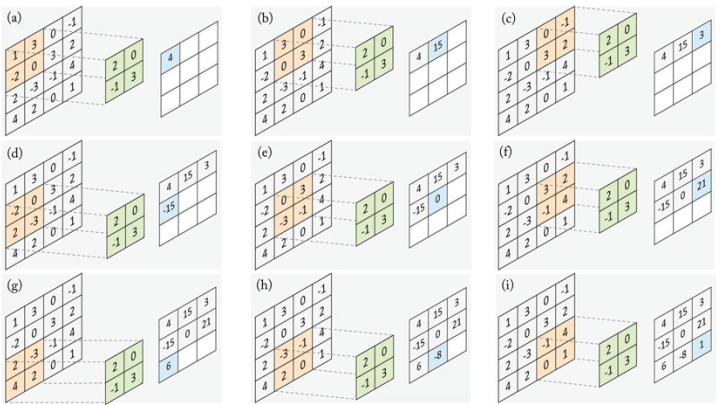
\includegraphics[width=1\textwidth]{filtro_de_red_convolucional}
	\caption[Ejemplo aplicación de un filtro.]{Ejemplo aplicación de un filtro\cite{cnn}.}
	\label{fig:filtro}
\end{figure}

Los pesos del filtro permanecen fijos a lo largo de la misma ejecución del algoritmo anterior aunque durante el entrenamiento se van ajustando a través de un proceso de retropropagación y descenso de gradiente.

Hay tres hiperparámetros que afectan al volumen de salida:

\begin{itemize}
	\item{Número de filtros}: afecta a la profundida de la salida, ya que cada filtro produce su mapa de características.
	
	\item{Stride}: es la distancia,  o el número de píxeles, que el kernel mueve sobre la matriz de entrada.
	
	\item{zero-padding}: Se utiliza para ajustar los filtros al tamaño de la imagen de entrada.
	pone a 0 todos los elemnetos que quedan fuera de la matriz de entrada. Hay tres tipos:
	
	\subitem{Valid padding}: O no padding, en este caso la última convolución se descarta si las dimensiones no se alinean.
	
	\subitem{Same padding}: Este garantiza que la capa de salida tenga el mismo tamaño que la de entrada. Es el utilizado en este trabajo.
	
	\subitem{Full padding}: Este aumenta el tamaño de la capa de salida añadiendo ceros en el borde de la entrada.
	
\end{itemize}

Después de cada convolución la red aplica una transformación de unidad lineal rectificada (ReLU) al mapa de características introduciendo no linealidad en el modelo. Esto eliminará los números negativos de este.
Después de una primera capa convolucional puede ir otra como ya se ha comentado.

\subsubsection{Capa de agrupación}
La agrupación de capas o submuestreo, permite reducir la dimensión mediante la reducción de los parámetros de la entrada. Este aplica una función de agregación a los valores dentro del campo receptivo y llena la matriz de salida.

Hay dos tipos de agrupación:
\begin{itemize}
	\item{Agrupación máxima}: a medida que recorre la entrada manda el pixel con el valor mayor a la matriz de salida.
	\item{Agrupación media}: a medida que recorre la entrada manda el valor medio de los pixeles dentro del campo receptivo a la matriz de salida
\end{itemize}

Aunque se pierde mucha información en la capa de agrupación esto ayuda a reducir la complejidad, mejora la eficiencia y limita el riesgo de sobreajuste. 

\subsubsection{Capa totalmente conectada}
Esta capa realiza la predicción en base a los mapas de características de las capas anteriores contra la imágen original. Suele usar una función softmax que clasifica valores de entre 0 y 1. En el caso de este experimento se utiliza una funcion sigmoid al ser una clasificación binaria.

\subsection{Red convolucional U-Net}
En este apartado explicaremos el funcionamiento de la red U-Net, un tipo de red convolucional muy utilizado para análisis de imágenes, el cual ha sido implementado en este experimento. Este es una mejora a otras redes convolucionales aumentando la precisión y pudiendo hacer clasificaciones más ajustadas.

Para comprender correctamente la arquitectura de la red U-Net\cite{Unet} es recomendable ver la figura~\ref{fig:red_U-Net}.

La red U-Net es una red neuronal convolucional qeu se divide en dos partes, el camino de expansión y el camino de compresión. La red empieza aplicando dos capas convolucionales a la imágen, separando en 64 mapas de características las imágenes y pasando a la siguiente capa estas además de pasandolo a la capa reflejada en el camino de expansión. La siguiente capa es una capa de agrupación, la cual se encarga de reducir su dimensionalidad. este proceso se repite en todo el camino de contracción. Una vez acaba el proceso de contracción se hace el proceso inverso para el proceso de expansión, sumando los mapas de características que se han obtenido en el camino de contracción.

\begin{figure}[H]
	\centering
	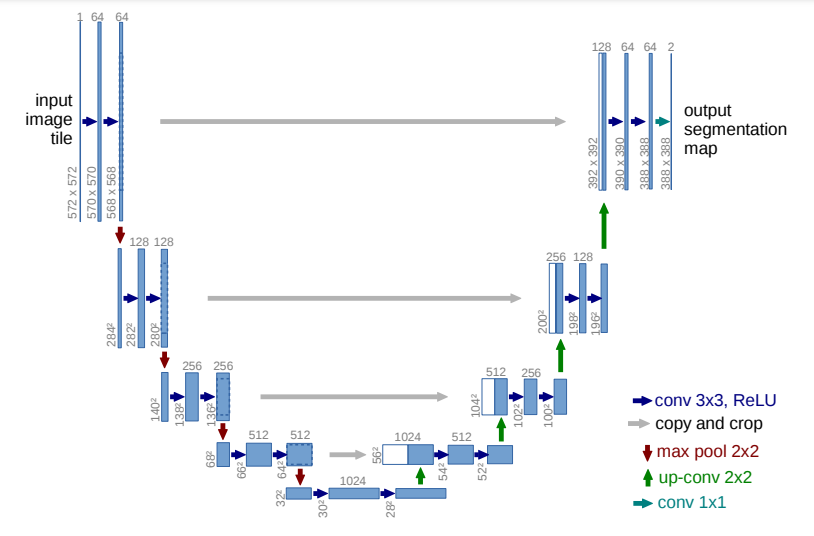
\includegraphics[width=1\textwidth]{red_U-Net}
	\caption[Funcionamiento red U-net.]{Funcionamiento red U-net\cite{Unet}.}
	\label{fig:red_U-Net}
\end{figure}
